% !TEX root = paper.tex

\section{Queries over Encrypted Data}
\label{s:design}


This section describes how \name{} executes SQL queries over encrypted
data.  The threat model in this section is threat 1 from
\S\ref{ss:dbthreat}; the DBMS machines and administrators are not
trusted, but the application and the proxy are trusted.
%(The next section
%removes these trust assumptions.)

\name{} enables the DBMS server to execute SQL queries on encrypted
data almost as if it were executing the same queries on plaintext
data. Existing applications do not need to be changed because the
proxy exports the same SQL interface as the DBMS\@. The DBMS's query
plan for an encrypted query is the same as for the original query.
However, the operators comprising the query, such as selections,
projections, joins, aggregates, and orderings, are performed on
ciphertexts, and use modified operators in some cases.

The \name{} proxy stores a secret master key, $\mathit{MK}$, and the database
schema.  The DBMS server sees an anonymized schema, encrypted user
data, and some auxiliary tables used by \name{}.  \name{} also equips
the DB server with \name{}-specific UDFs that enable the server to
compute on ciphertexts for certain operations.

Processing a query in \name{} involves four steps:
\begin{CompactEnumerate}
\item The application issues a query, which the proxy intercepts and
  rewrites: it anonymizes each table and column name, and, using the
  master key $\mathit{MK}$, encrypts each constant in the query with an
  encryption scheme best suited for the desired operation
  (\S\ref{ss:sqlaware}).
\item The proxy passes the query to its {\em onion key manager (OKM)}
  module, which assesses if the server should be given onion keys to
  execute the query. If so, the OKM does so by issuing an
  \texttt{UPDATE} query at the server that invokes a UDF to adjust the
  privacy level of the appropriate columns (\S\ref{ss:onion}).
\item The proxy forwards the encrypted query to the DBMS server,
  which executes it using standard SQL (occasionally invoking 
  UDFs for aggregation).
\item The DBMS server returns the query result, which the proxy
  decrypts and returns to the application.
\end{CompactEnumerate}

%To execute each SQL query, the proxy anonymizes, encrypts and rewrites
%the query before forwarding it to the untrusted DBMS server.  
% To anonymize a query, the proxy replaces each table with the table
% name from the anonymized schema (see Figure \ref{fig:schema}).  
% For
% projection, the proxy replaces each column with the name of the
% anonymized column for the first onion.  

\subsection{SQL-aware Encryption}
\label{ss:sqlaware}

The key idea to our design is that different encryption schemes enable
different SQL operations.  We use existing encryption schemes, optimize
a recent scheme, and design a new cryptographic primitive for joins.

\name{} uses the same key (derived from $\mathit{MK}$) to encrypt each  data item in a column so that the same computation can be performed on every
element in that column. (We will
  use finer-grained encryption in \S\ref{s:multi} to reduce the
  potential damage of application compromise.)

For each encryption type we use, we explain the security property that
\name{} requires from it, its functionality, and how to implement it with existing schemes. 
 
\textbf{Random} ($\RND$)\@. $\RND$ provides maximum security:
indistinguishability under an adaptive chosen-ciphertext attack
(IND-CCA2).  Two equal values will be
mapped to different encryptions with high probability. $\RND$ does not
allow any computation to be performed efficiently on the ciphertext.
To implement $\RND$, \name{} uses AES in UFE mode~\cite{desai:ufe}.

\textbf{Deterministic} ($\DET$)\@. $\DET$ has a slightly weaker
guarantee, yet is still has strong security: it only leaks which encrypted values correspond to the same
data value. This encryption level allows the server to perform
equality checks, which means it can perform selects with equality
filters, equality joins, {\tt GROUP BY}, {\tt COUNT}, {\tt DISTINCT},
etc.  There are
many ways to implement $\DET$, such as $\DET_K(v)=\RND_{K_1}(v) ~ \| ~
\textrm{HMAC-SHA1}_{K_2}(v)$, where $\|$ is the
concatenation operator, $K_1$ and $K_2$ are two keys derived from $K$,
and $K$ itself is derived by encrypting the table and column names
with $\mathit{MK}$\@.  For this $\DET$ construction, the server compares two
encryptions by comparing their HMAC-SHA1
values.
% We implement $\DET$ using AES in counter mode with a
% separate IV (counter value) for each column, derived by encrypting the table
% and column names with $\MK$\@.

\textbf{Order-preserving encryption} ($\OPE$)\@. $\OPE$ allows order
relations between data items to be established based on their
encrypted values, but does not leak any other information about the
data. If $x < y$, then $\OPE_K(x) < \OPE_K(y)$, for any secret key $K$\@.
Therefore, if a column is encrypted with $\OPE$, the server can
perform range queries when given encrypted constants $\OPE_K(c_1)$ and
$\OPE_K(c_2)$ corresponding to the range $[c_1, c_2]$.  The server can
also perform {\tt ORDER BY}, {\tt MIN}, {\tt MAX}, {\tt SORT}, etc.

$\OPE$ is a weaker encryption scheme than $\DET$ because it reveals
order.  Thus, the \name{} proxy will only reveal $\OPE$-encrypted
columns to the server if users request order queries on those
columns. $\OPE$ has provable security guarantees~\cite{boldyreva-ope}: the encryption is
equivalent to a random permutation that preserves order.  Therefore,
the difference between two encryptions $\OPE_K(y) - \OPE_K(x)$ is
basically random, and reveals no information about $y - x$ except for
the sign.

The scheme we use~\cite{boldyreva-ope} is the first provably secure
scheme.  Until \name{}, there has not been an implementation or any
measure of how practical the scheme would be.  The direct
implementation of the scheme took $\sim$25~ms per encryption.  We
improved the algorithm by using AVL binary search trees when batch
encryption is done (e.g., database loads), reducing the cost of $\OPE$
encryption to 7~ms per encryption without affecting its security. We
also implemented a hypergeometric sampler that lies at the core of
$\OPE$, porting a Fortran implementation from 1988~\cite{HGD88}.

% We implemented several optimizations to reduce its cost.
% At a high-level, given a value $v$, $\OPE$ performs binary search in
% he field of encryptions to find an encryption for $v$.  
% Caching
% intermediate search results for reuse across encryptions
% of different values improves performance of batch operations, such
% as database loads.  
% We use AVL binary search trees to perform
% efficient cache lookups.  


% The most efficient such scheme was proposed in $1988$ (now
% used in tools such as MathWorks); we translated its
% original implementation from Fortran-1988.

\textbf{Homomorphic encryption} ($\HOM$)\@. $\HOM$ is a highly secure
encryption scheme (IND-CCA secure), allowing the server to perform
computations on encrypted data with the final result decrypted at the
proxy. While fully-homomorphic encryption is prohibitively
slow~\cite{trillion}, homomorphic encryption for specific operations
is efficient.  To support summation, we implemented the Paillier
cryptosystem~\cite{Paillier99}.  With Paillier, multiplying the
encryptions of two values results in an encryption of the sum of the
values, i.e., $\HOM_K(x) \cdot \HOM_K(y) = \HOM_K(x+y)$, where
multiplication is performed modulo some public-key value.  To compute
{\tt SUM} aggregates, \name's proxy replaces {\tt SUM} with calls to a
UDF that performs Paillier multiplication on a column encrypted with
$\HOM$.  $\HOM$ can also be used for computing averages by having the
DBMS server return the sum and the count separately, and for
incrementing values (e.g., {\tt SET id=id+1}), on which we will
elaborate shortly.

In $\HOM$, the ciphertext is 2048 bits; however, we can pack
multiple values into one ciphertext using the scheme
of~\cite{GeZ07}, with an amortized space overhead of only 2 times
(e.g., a 32-bit value occupies 64 bits).

\textbf{Word search} ($\SEARCH$)\@.  To allow word searches in a given
column (e.g., using the MySQL ``ILIKE'' operator), we implement a
cryptographic protocol for keyword searches on encrypted
text~\cite{Dawn-Song-Search-2000, amanatidis-boldyreva-o'neill}.
%$\SEARCH$ allows the server to detect repeating words in a given
%column.

\textbf{Join} ($\JOIN$ and $\OPEJOIN$)\@.  A separate encryption
is necessary to allow equality joins between two columns, because we
use different keys for $\DET$ to prevent cross-columns correlations.   $\JOIN$ also supports all operations allowed by $\DET$ and
$\SEARCH$, and also allows the server to detect repeating values
between two columns.  $\OPEJOIN$ enables joins by order relations. We provide a new cryptographic scheme for join and we discuss it in \S\ref{ss:join}.

\begin{figure}[t!]
\centering
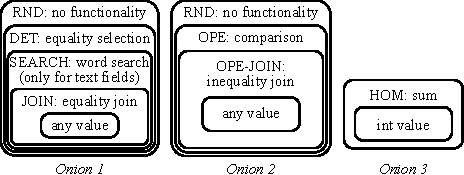
\includegraphics{fig/storage2.pdf}
\caption{Onion layers of encryption and the classes of computation they allow.}
\label{fig:onion}
\end{figure}

\name{} uses existing transaction and indexing mechanisms in the DBMS
server without any modifications.  For transactions, the proxy passes
along any {\tt BEGIN}, {\tt COMMIT}, and {\tt ABORT} queries to the
DBMS\@.
The DBMS builds indexes of encrypted columns in the same way as it
builds indexes of plaintext data.  The proxy does not request indexes
on $\RND$ encryptions, since no lookups are performed at that level,
but the DB server can construct indexes on $\DET$, $\JOIN$, $\OPE$, and
$\OPEJOIN$ encryptions, as with unencrypted data.
% if the application's schema requested an
% index on the corresponding column (e.g., using an {\tt ALTER} or
% {\tt CREATE} query).

\subsection{Adjustable Query-based Encryption}
\label{ss:onion}

A key part of \name{}'s design is \textit{adjustable query-based
  encryption}, which dynamically adjusts the level of encryption on
the DBMS server.  The goal is provide the most secure encryption
scheme that can also run each query.  For example, if there
is no reason to compare data items in a column, or sort a column, the
column should be encrypted with $\RND$, and for columns that perform
equality checks but not inequality checks, $\DET$ suffices.
Unfortunately, the query set is not always known in advance.
Thus, we need an adaptive scheme that dynamically
adjusts encryption strategies.

Our idea is to encrypt each data item into an \textit{onion}:
each value in the table is dressed in layers of increasingly stronger
encryption, as illustrated in Figs.~\ref{fig:onion} and~\ref{fig:schema}. Each layer of
each onion enables certain kinds of functionality as explained in the
previous subsection.  For example, the outermost layers, $\RND$ and
$\HOM$, provide maximum security, whereas $\OPE$ provides more
functionality.  For numeric values, \name{} maintains three onions,
and for string values, \name{} maintains two onions (the $\DET$ onion,
of the same length as the string, the $\OPE$ onion, of constant length,
and no $\HOM$ onion).

%To prevent the server from learning information from column or table
%names, \name{}'s proxy also anonymizes the schema.

For each level of each onion, the proxy uses the same key for
encrypting values in the same column, and different keys across
columns, onion levels, and tables.  All these keys are derived from
the master key $\mathit{MK}$\@.  For example, for table $t$, column $c$,
encryption level $l$, the proxy uses the key
\begin{equation}\label{eq:columnkey}
K_{t, c, l} = \textrm{PRP}_\mathit{MK} (\mathrm{table}\>t, \mathrm{column}\>c,
    \mathrm{level}\>l),
\end{equation}
where PRP is a pseudorandom permutation (e.g., AES).

Each onion starts out encrypted with the most secure encryption scheme
($\RND$ for onions 1 and 2, and $\HOM$ for onion 3)\@.  As the proxy
receives SQL queries from the application, the onion key manager (OKM)
determines whether layers of encryption need to be removed.  Given a
predicate $P$ on column $c$ needed for the query, the OKM first
establishes what onion layer is needed to perform $P$ on $c$.  If the
encryption of $c$ is not already at an onion layer that allows $P$,
the OKM strips off the onion layers to allow $P$ on $c$, by sending
the corresponding onion key to the server. The lowest encryption level is never stripped.

\name{} implements onion layer decryption using UDFs that run on the
DBMS server.  For example, in Fig.~\ref{fig:schema}, to decrypt onion 2 of column 2 in table 1 
to level $\OPE$, the OKM issues the following query to the server
using the {\tt DECRYPT\_RND} UDF:

\begin{verbatim}
 UPDATE Table1 SET C2-Onion2 =
                   DECRYPT_RND(K, C2-Onion2)
\end{verbatim}
where $K$ is the appropriate key computed as in Eq.
(\ref{eq:columnkey}).

Each constant in a query that is part of a predicate on onion $o$ of column $c$ is encrypted using all onion layers up to the current onion layer of onion $o$ of column $c$. 

Note that onion decryption is performed entirely by the DBMS server.
In the steady state, {\em no server-side decryptions are needed},
because onion decryption happens only when a new type of computation
is performed on a column.  For example, after an equality check is performed
on a column and the server brings the column to level $\DET$, the
column remains in that state, and future queries with equality checks require no decryption.  This property ensures that the
overhead of \name{} is modest in the steady state (see \S\ref{s:eval}) because the server mostly performs typical SQL processing.
The security level to which the database converges is the maximum
privacy level for the set of queries issued by the application.

\newcommand\B{\rule[-2.0ex]{0pt}{0pt}}

\begin{figure}[t!] 
\scriptsize
\begin{minipage}[h]{0.6in}
\begin{tabular}{@{~~}c@{~~}|@{~~}c@{~~}}
\multicolumn{2}{@{~}c@{~}}{\bf Employees\B} \\
ID & Name \\ \hline
23 & Alice \\
\end{tabular}
\end{minipage}
%
\begin{minipage}[h]{0in}
\begin{tabular}{@{~}c@{~}|@{~}c@{~}|@{~}c@{~}||@{~}c@{~}|@{~}c@{~}}
\multicolumn{5}{@{~}c@{~}}{\bf Table1\B} \\
C1-Onion1 & C1-Onion2 & C1-Onion3 & C2-Onion1 & C2-Onion2 \\ \hline
x2b82ae & xcb9e4 & xc234e4 & x8ab113 & xd101e3 \\
\end{tabular}
\end{minipage}

\caption{Data layout at the server. When the application creates a
  table with the schema on the left, the table created at the server
  is the one from the right.}
\label{fig:schema}
\end{figure}


\paragraph{Read Query Execution.}

Consider an example consisting of a table \texttt{Employees}, which
has four columns of interest: \texttt{id}, \texttt{name},
\texttt{address}, and {\tt salary}.  Initially, each column in the
table is dressed in all onions of encryption, with $\RND$ and $\HOM$
as outermost layers, as shown in Figure~\ref{fig:onion}.  At this
point, the server can learn nothing about the data content other than
the number of columns, rows, and data size.

To execute predicates on a column, the proxy replaces the column with the
name of the onion that allows the necessary operation on
that field, and, for certain operations (such as {\tt SUM}), the proxy
replaces the operation with its equivalent UDF that operates on
ciphertexts.  

To illustrate when onion layers are removed, consider the query
\texttt{SELECT * FROM Employees WHERE name = 'Alice'}, which requires
lowering encryption of {\tt name} to level $\DET$\@.  In this case,
the proxy first issues the query \texttt{UPDATE Table1 SET C2-Onion1 =
  DECRYPT\_RND($K_{1,2,\RND}$, C2-Onion1)}, and then \texttt{SELECT
  C1-Onion1, C2-Onion1, C3-Onion1, C4-Onion1 FROM Table1 WHERE
  C2-Onion1 = x7d35a3}, where \texttt{x7d35a3} is an encryption of
``Alice'' with key $K_{1,2,\DET}$\ and the keys for lower onion layers.  The proxy decrypts the results
from the server and returns them to the user.

If the next query is {\tt SELECT COUNT(*) FROM Employees WHERE name =
  'Bob'}, no server-side decryptions are necessary, and the proxy
directly issues the query {\tt SELECT COUNT(*) FROM Table1 WHERE
  C2-Onion1 = xbb234a}, where \texttt{xbb234a} is the encryption of ``Bob''.

% Finally, the proxy replaces aggregation operators with equivalent UDFs
% that operate on encrypted values.  For example, if the user issues the
% query {\tt SELECT SUM(salary) FROM Employees}, the proxy rewrites it
% to {\tt SELECT HOM\_AGG(C4-Onion3, PKTABLE.PK) FROM Table2}, where
% {\tt HOM\_AGG} is a UDF that performs Paillier multiplication
% (resulting in addition of plaintexts), {\tt PKTABLE} is a table of
% public keys \name{}{} stores at the server (see
% Fig.~\ref{fig:overview}), and $\PK$ is the Paillier public key
% modulus.


\paragraph{Write Query Execution.}

To support {\tt INSERT}, {\tt DELETE}, and {\tt UPDATE} queries, the
\name{} proxy applies the same processing to the predicates (i.e., the
{\tt WHERE} clause) as for read queries.  {\tt DELETE} queries require
no additional processing.  For all {\tt INSERT} queries and for {\tt
  UPDATE} queries that set the value of a column to a constant, the
proxy encrypts each inserted column's value with each onion layer that
has not been stripped off yet in that column
%For {\tt UPDATE} queries that set the value of a column to a constant,
%the proxy encrypts the value in the appropriate onions as for {\tt
%  INSERT}.

The remaining case is an {\tt UPDATE} that sets a column value based
on another column value, such as {\tt salary=salary+1}.  Such an
update would have to be performed using $\HOM$, to handle additions.
However, in doing so, the values in the $\OPE$ and $\DET$ onions would
become stale.  In fact, an encryption scheme that allows both addition
and comparison at the same time is fundamentally insecure: if a
malicious server knows the order of the items ($\OPE$) and can
increment the value by one, the server can keep adding one to each
field homomorphically until the field becomes equal to some other
value.  This would allow the server to compute the difference between
any two values in the database, which is almost equivalent to knowing
their values.

There are two solutions to this problem.  If a column is incremented
and then only projected (no comparisons performed on it), the solution
is simple: when requesting the value of this field, use the value of
Onion 3 rather than Onion 1 or 2, because Onion 3 is up-to-date.  This
is the case for increment TPC-C queries.
If a column is used in comparisons after it is
incremented, the solution is to split the query into two parts:
a select of the old values to be updated, and an update using
the new values. 
This strategy works well in practice (such as in TPC-C and our benchmark
applications) because updates are typically executed on either individual
rows or a small number of rows.

% removed for space
%.  That is,
% for query \texttt{UPDATE Employees SET salary=salary+1 WHERE id=3},
% the proxy issues the encrypted version of \texttt{SELECT salary FROM
%  Employees WHERE id=3}, and then the encrypted version of
%\texttt{UPDATE Employees SET salary=z WHERE id=3}, where $z$ is one
% more than the result of the first query.\footnote{If the first {\tt
%    SELECT} query returns more than one result, the proxy computes a
%  mapping of old encrypted {\tt salary} values and the corresponding
%  new encrypted {\tt salary} values, and uses a UDF in the second {\tt
%    UPDATE} query to update the {\tt salary} column according to this
%  mapping.}  However, in most cases in practice (such as in TPC-C),
% such updates are executed on individual rows.

\subsection{Computing Joins}
\label{ss:join}

There are two kinds of joins: {\em equi-joins} in which
the join predicate is based on equality, and {\em range joins}, which
involve order checks.
Supporting these joins is a challenging problem.  If two columns are
to be joined, they need to be encrypted with the same key.

% We first describe how \name{} implements
% equi-joins (the overwhelmingly common case, i.e., level
% $\JOIN$), and then describe inequality joins (level $\OPEJOIN$).

%We first describe how \name{} implements equi-joins.  

To provide maximum privacy for equi-joins, the DBMS server should not
be able to join columns for which the user did not request a join, so
columns that are never joined should not be encrypted with the same
keys.  Moreover, if users request a join of columns $A$
and $B$, and a join of columns $C$ and $D$, the DBMS server should not
be able to join $B$ and $C$\@.  Thus, the question is, which keys
should each column be encrypted with, given that we do not know in
advance what columns will be joined?

To address this problem, we introduce a new cryptographic primitive
that allows the DBMS server to dynamically adjust the $\JOIN$
encryption keys of each column.  Each column is initially encrypted
with a different $\JOIN$ key, preventing all joins.  When a query
requests a join, the proxy will give the DBMS server an onion key to
re-encrypt the two columns to the same $\JOIN$ key, allowing joins
between the two columns.

Our algorithm is based on elliptic-curve cryptography (ECC).  When a
row is inserted, the $\JOIN$ encryption of value $v$ is computed as
$\JOIN_K(v) := H(v)^K$, where $K$ is the initial key for that table,
column, and level, and $H$ is a mapping from values (integers or
strings) to a point on an elliptic curve.  When the query joins columns $c$ and
$c'$, the proxy computes $\Delta K=K/K'$, which can be used to bring
the $\JOIN$ encryptions of $c$ and $c'$ to the same key.  Given
$\JOIN_{K'}(v)$ (stored in column $c'$) and $\Delta K$, the DBMS
server uses a UDF to compute $\JOIN_{K'}(v)^{\Delta K} =
H(v)^{K'\times K / K'} = H(v)^K = \JOIN_K(v)$.  Now columns $c$ and
$c'$ share the same $\JOIN$ key, and the DBMS server can perform an
equi-join on $c$ and $c'$ as usual.

We proved the security of this scheme cryptographically (elided here
for space, but will be in an extended version) using the hardness
assumption of computing the discrete logarithm in elliptic curve-based
groups. The server can only join pairs of columns that were joined by
a legitimate query and the encryption scheme does not reveal data.
% 5Intuitively,
% the server cannot perform an equi-join without knowing $K/K'$, and
% $K/K'$ does not reveal any information about either $K$ or $K'$.
% Moreover, the server cannot compute $K$ from $H(v)^K$ because of the
%Given two columns encrypted with $K$
%and $K'$, if the server is not given $K/K'$, it cannot bring the two
%columns to the same encryption level, and thus cannot perform
%unrequested joins.
% We use ECC because of it is
% relatively efficient and ciphertexts are small ($\approx 160$ bits) compared to ciphertexts in
% typical public key cryptosystems for the same security
% level.

% : computing $\JOIN_{K'}(v)^{K/K'}$ is basically a
% multiplication, and does not involve any exponentiation; moreover, ECC

For range joins, a similar dynamic re-encryption scheme is difficult
to construct due to lack of structure of $\OPE$ schemes.  Instead,
\name{} requires that pairs of columns that will be involved in such
joins be declared by the application ahead of time, so that matching
keys are used for level $\OPEJOIN$ of those columns.  Fortunately,
range joins are rare (and not used in any of our example
applications).
%Alternatively, level $\OPEJOIN$
%encryptions can be re-encrypted with matching keys at the expense of
%sending an entire column to the proxy for re-encryption, and then
%sending it back to the DBMS server.

\subsection{Optimizations}
\label{ss:optimize}

\name{} implements four performance optimizations.

\textbf{Insensitive fields.} By default, \name{} encrypts all fields. 
The programmer can annotate just the sensitive fields in the schema
(\S\ref{sec:multi}) to avoid encrypting public fields.

\textbf{Known query set.}  If an application has a known query set or a set of queries likely to happen, as is the case for many web applications, \name{} has a training module that can adjust onions at this level before system startup, thus reducing onion adjustment work from runtime. For a fully known query set, \name{} can also discard any onions that will not be needed (e.g., discard $\OPE$ onion for a column if range queries are not performed on that column).

% For many applications, the queries issued
%by the application are fixed and known ahead of time.  In this case,
% we do not need to adjust onion levels at runtime, and can start the
% database with the exact onion encryption levels that we need.
% Moreover, if a certain column is never used in certain operations, the
%corresponding onion can be omitted altogether.  For example, if an
% application never performs range or order operations on a column, the
% $\OPE$ onion for that column can be omitted.  Discarding onions
% significantly reduces performance costs both in the proxy and in the
% DBMS server.  This optimization is implemented by a \textit{train}
% module in the proxy, which, given a set of queries a user application
% will issue, determines the exact levels of encryption needed.

\textbf{Security convergence.}  Even if the query set is not known in
advance, after an application has run for a considerable time, the
proxy may drop any onions that have not been used, because these
onions are unlikely to be used in the future.  If a query does happen
to use these onions later, the proxy can go through the cost of
adding back the deleted column, but such event should be rare.

\textbf{Ciphertext caching.}  A significant ongoing cost for the proxy
lies in generating $\OPE$ and $\HOM$ encryptions of constants used in
queries.  To avoid this cost, the proxy maintains a cache of
commonly-used constants, along with their encryptions under different
keys.  Since some constants are repeatedly used in queries (e.g.,
the constant 1), this optimization reduces the amount of CPU time
spent by the proxy encrypting data.

\subsection{Discussion}

\name{}'s design supports most relational queries and aggregates on
standard data types, such as integers and text/varchar types.
Additional operations can be added to \name{} by extending its
existing onions, or adding new onions for specific data types (e.g.,
spatial and multi-dimensional range
queries~\cite{multidimRangeQueries}).

There are certain computations \name{} cannot support on encrypted
data. For example, it does not support both computation and comparison
on the same column, such as \texttt{WHERE salary > age*2+10}.  \name{}
can process a part of this query, but it would also require some
processing on the proxy.  In \name{}, such a query should be (1)
rewritten into a sub-query that selects a whole column, \texttt{SELECT
  age*2+10 FROM $\ldots$}, which \name{} computes using $\HOM$, and
(2) re-encrypted in the proxy, creating a new column (call it {\tt
  aux}) on the DBMS server consisting of the newly-encrypted values.
Finally, the original query with the predicate {\tt WHERE salary >
  aux} should be run.  We have not been affected by this limitation in
our test applications (TPC-C, phpBB, HotCRP, and grad-apply).
%Nevertheless, as we will
%see from \S~\ref{s:eval}, \name{}{} supports all queries on TPC-C and
%queries on sensitive data we have encountered in real applications.

%The current \name{} prototype does not support stored procedures or
% other user-defined functions on the server.  Supporting stored
% procedures written in SQL should be straightforward, by having the
% proxy rewrite the SQL statements inside of the stored procedure
%as it would for any other query.  On the other hand, \name{}'s
%design cannot support the execution of arbitrary user-defined
%functions (not written in SQL) over encrypted data.

% \subsection{Access Control}
% 
% Access control can be implemented at the proxy or at a machine between the
% users and the front end. There has been significant work done on such schemes
% which can be used with \name{}. 



